\section{Preventivo} %Meccanismi di controllo e rendicontazione
Viene in seguito presentato il preventivo del costo del lavoro da svolgere con i dettagli sul costo di ogni singolo periodo.
Per identificare i diversi ruoli verranno utilizzate le sigle:
\begin{itemize}
	\item \textbf{Re}: responsabile di progetto\glo;
	\item \textbf{Am}: amministratore di progetto\glo;
	\item \textbf{An}: analista;
	\item \textbf{Pt}: progettista;
	\item \textbf{Pr}: programmatore;
	\item \textbf{Ve}: verificatore.
\end{itemize}
	\subsection{Periodo di analisi}
	Le ore indicate per questo periodo vengono riportate solo perché utili ai fini del documento, non saranno rendicontate nel budget finale richiesto in quanto il periodo di analisi è da considerare come investimento per il gruppo.
	\pagebreak
		\subsubsection{Prospetto orario}
		Nel periodo di analisi è prevista la seguente divisione oraria:
		\begin{longtable} {				
				>{}p{40mm}  
				>{}p{8mm}
				>{}p{8mm}
				>{}p{8mm}
				>{}p{8mm}
				>{}p{8mm}
				>{}p{8mm}
				>{}p{12mm}				
			}			
			\rowcolor{gray!50}
			\textbf{Nominativo} & \textbf{Re} & \textbf{Am} & \textbf{An} & \textbf{Pt} & \textbf{Pr} & \textbf{Ve} & \textbf{Totale}	\TBstrut \\ [2mm]
			Corrizzato Vittorio & 6 & 6 & 8 & - & - & 5 & 25 \TBstrut \\ [2mm]
			Dalla Libera Marco & 7 & - & 13 & - & - & 5 & 25 \TBstrut \\ [2mm]
			Rampazzo Marco & - & 8 & 12 & - & - & 5 & 25 \TBstrut \\ [2mm]
			Santagiuliana Vittorio & - & 5 & 12 & - & - & 8 & 25 \TBstrut \\ [2mm]
			Schiavon Rebecca & - & - & 15 & - & - & 10 & 25 \TBstrut \\ [2mm]
			Spreafico Alessandro & - & - & 12 & 5 & - & 8 & 25 \TBstrut \\ [2mm]
			Toffoletto Massimo & 8 & 7 & 5 & - & - & 5 & 25 \TBstrut \\ [2mm]
			\rowcolor{white}
			\caption{Prospetto orario del periodo di analisi}
		\end{longtable}
		Rappresentata nel seguente grafico:
		\begin{figure} [H]
			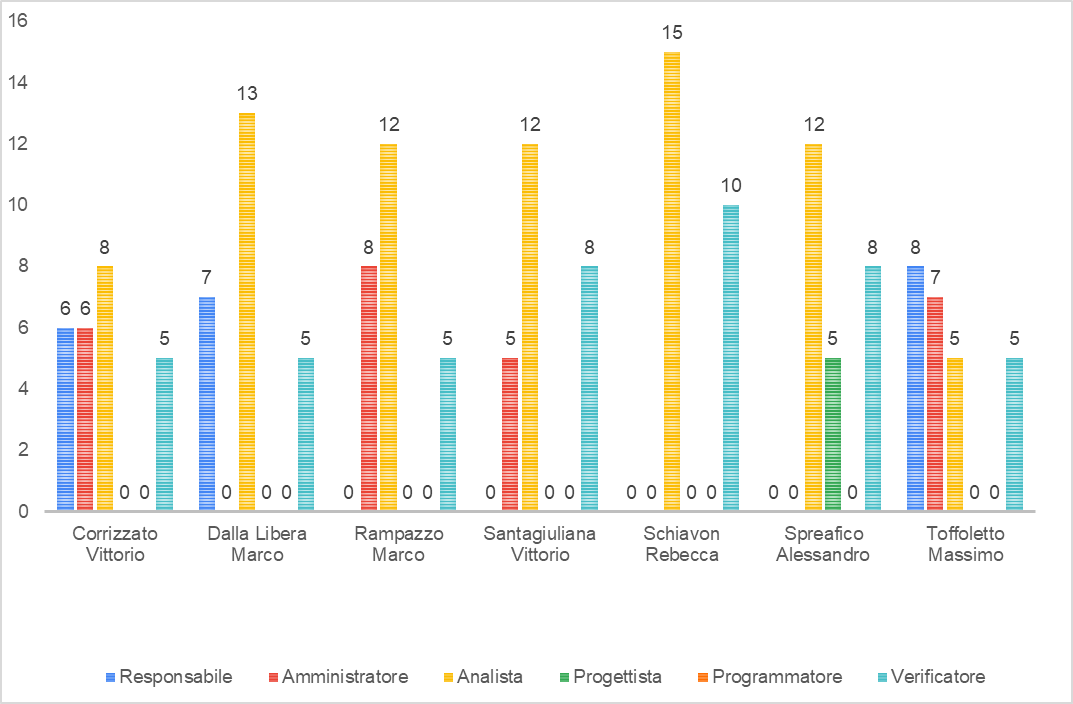
\includegraphics[width=\linewidth]{./img/Grafici/1.png}
			\caption{Grafico del prospetto orario del periodo di analisi}
		\end{figure}
	
		\subsubsection{Prospetto economico}
		Nel periodo di analisi sono previsti i seguenti costi:
		\begin{longtable} {
			>{}p{32mm}
			>{}p{20mm}
			>{}p{20mm}
		}
		\rowcolor{gray!50}
		
		\textbf{Ruolo} & \textbf{Ore} & \textbf{Costo} \TBstrut \\
		Responsabile & 21 & 630,00\euro{} \TBstrut \\
		Amministratore & 26 & 520,00\euro{} \TBstrut \\
		Analista & 77 & 1925,00\euro{} \TBstrut \\
		Progettista & 5 & 110,00\euro{} \TBstrut \\
		Programmatore & 0 & 0,00\euro{} \TBstrut \\
		Verificatore & 46 & 690,00\euro{} \TBstrut \\
		\textbf{Totale} & \textbf{175}& \textbf{3875,00\euro{}} \TBstrut \\
		\rowcolor{white}
		\caption{Prospetto economico del periodo di analisi}		
		\end{longtable}
		Rappresentati nel seguente grafico:
		\begin{figure} [H]
			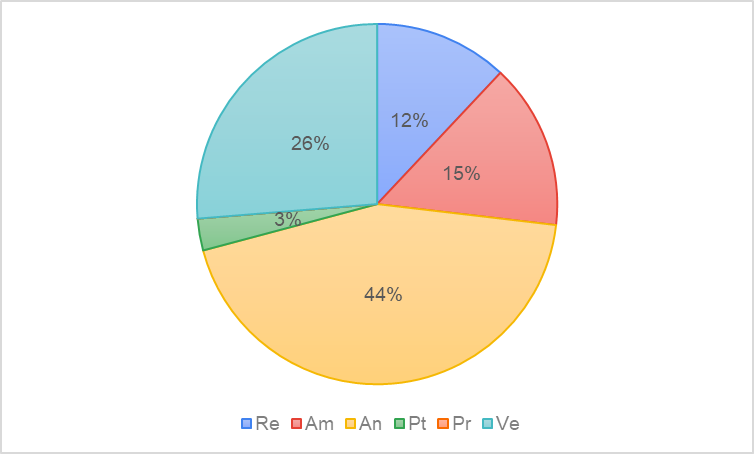
\includegraphics[width=\linewidth]{./img/Grafici/2.png}
			\caption{Grafico del prospetto economico del periodo di analisi}
		\end{figure}
\subsection{Periodo di progettazione architetturale}
	\subsubsection{Prospetto orario}
	Nel periodo di progettazione\glosp architetturale è prevista la seguente divisione oraria:
	\begin{longtable} {				
		>{}p{40mm}  
		>{}p{8mm}
		>{}p{8mm}
		>{}p{8mm}
		>{}p{8mm}
		>{}p{8mm}
		>{}p{8mm}
		>{}p{12mm}				
	}			
	\rowcolor{gray!50}
	\textbf{Nominativo} & \textbf{Re} & \textbf{Am} & \textbf{An} & \textbf{Pt} & \textbf{Pr} & \textbf{Ve} & \textbf{Totale}	\TBstrut \\ [2mm]
	Corrizzato Vittorio & - & - & 6 & 10 & 5 & 7 & 28 \TBstrut \\ [2mm]
	Dalla Libera Marco & - & 5 & 7 & - & 7 & 9 & 28 \TBstrut \\ [2mm]
	Rampazzo Marco & 6 & - & - & 9 & 8 & 5 & 28 \TBstrut \\ [2mm]
	Santagiuliana Vittorio & - & - & - & 14 & 5 & 9 & 28 \TBstrut \\ [2mm]
	Schiavon Rebecca & 7 & - & - & - & 9 & 12 & 28 \TBstrut \\ [2mm]
	Spreafico Alessandro & - & 5 & 5 & - & 10 & 8 & 28 \TBstrut \\ [2mm]
	Toffoletto Massimo & - & - & 6 & 5 & 7 & 10 & 28 \TBstrut \\ [2mm]
	\rowcolor{white}
	\caption{Prospetto orario del periodo di progettazione\glosp architetturale}
	\end{longtable}
	\pagebreak
	Rappresentata nel seguente grafico:
	\begin{figure} [H]
		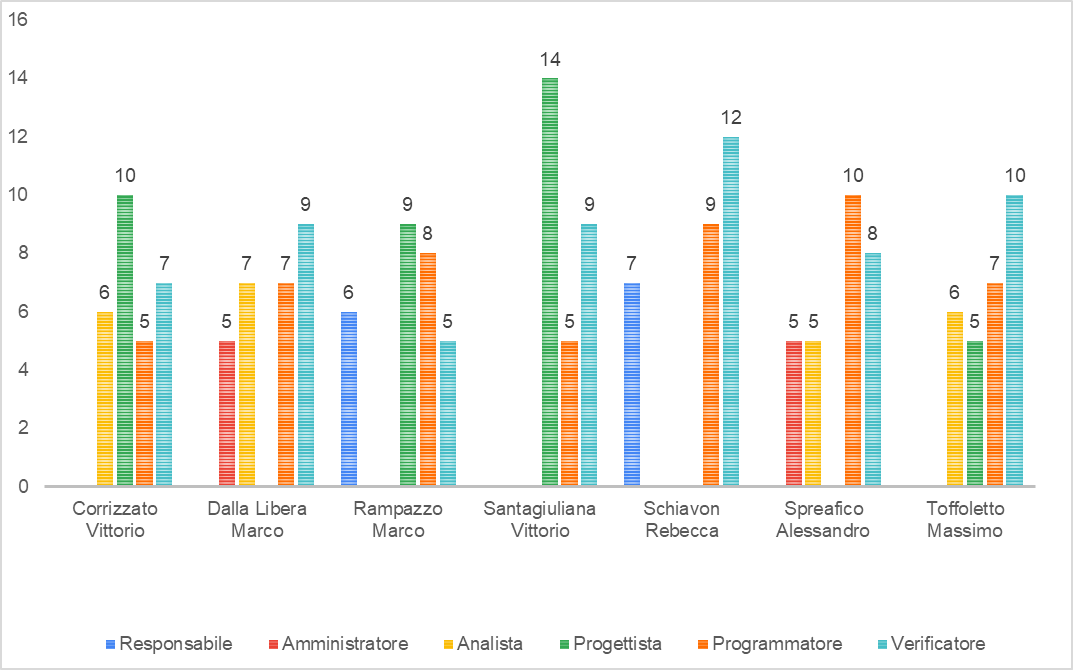
\includegraphics[width=\linewidth]{./img/Grafici/3.png}
		\caption{Grafico del prospetto orario del periodo di progettazione\glosp architetturale}
	\end{figure}

\subsubsection{Prospetto economico}
Nel periodo di progettazione\glosp architetturale sono previsti i seguenti costi:
\begin{longtable} {
		>{}p{32mm}
		>{}p{20mm}
		>{}p{20mm}
	}
	\rowcolor{gray!50}
	
	\textbf{Ruolo} & \textbf{Ore} & \textbf{Costo} \TBstrut \\
	Responsabile & 13 & 390,00\euro{} \TBstrut \\
	Amministratore & 10 & 200,00\euro{} \TBstrut \\
	Analista & 24 & 600,00\euro{} \TBstrut \\
	Progettista & 38 & 836,00\euro{} \TBstrut \\
	Programmatore & 51 & 765,00\euro{} \TBstrut \\
	Verificatore & 60 & 900,00\euro{} \TBstrut \\
	\textbf{Totale} & \textbf{196}& \textbf{3691,00\euro{}} \TBstrut \\	
	\rowcolor{white}
	\caption{Prospetto economico del periodo di progettazione architetturale}
\end{longtable}
\pagebreak
Rappresentati nel seguente grafico:
\begin{figure}[H] 
	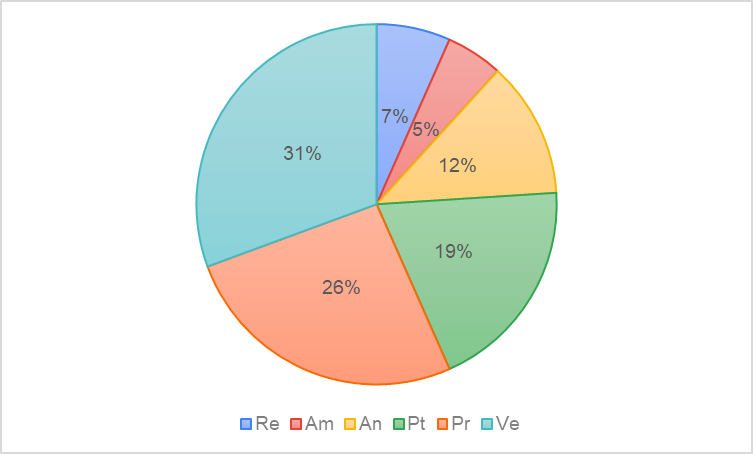
\includegraphics[width=\linewidth]{./img/Grafici/4.png}
	\caption{Grafico del prospetto economico del periodo di progettazione\glosp architetturale}
\end{figure}
\pagebreak
\subsection{Periodo di progettazione dettaglio e codifica}
\subsubsection{Prospetto orario}
Nel periodo di progettazione\glosp dettaglio e codifica è prevista la seguente divisione oraria:
\begin{longtable} {				
		>{}p{40mm}  
		>{}p{8mm}
		>{}p{8mm}
		>{}p{8mm}
		>{}p{8mm}
		>{}p{8mm}
		>{}p{8mm}
		>{}p{12mm}				
	}			
	\rowcolor{gray!50}
	\textbf{Nominativo} & \textbf{Re} & \textbf{Am} & \textbf{An} & \textbf{Pt} & \textbf{Pr} & \textbf{Ve} & \textbf{Totale}	\TBstrut \\ [2mm]
	Corrizzato Vittorio & - & - & 9 & 23 & 22 & - & 54 \TBstrut \\ [2mm]
	Dalla Libera Marco & 9 & - & 6 & 15 & 15 & 9 & 54 \TBstrut \\ [2mm]
	Rampazzo Marco & - & 5 & - & 23 & 18 & 8 & 54 \TBstrut \\ [2mm]
	Santagiuliana Vittorio & 8 & - & - & 20 & 15 & 11 & 54 \TBstrut \\ [2mm]
	Schiavon Rebecca & - & - & 8 & 20 & 18 & 8 & 54 \TBstrut \\ [2mm]
	Spreafico Alessandro & 8 & - & 0 & 16 & 18 & 12 & 54 \TBstrut \\ [2mm]
	Toffoletto Massimo & - & 5 & - & 23 & 15 & 11 & 54 \TBstrut \\ [2mm]
	\rowcolor{white}
	\caption{Prospetto orario del periodo di progettazione\glosp dettaglio e codifica}
\end{longtable}
\pagebreak
Rappresentata nel seguente grafico:
\begin{figure} [H]
	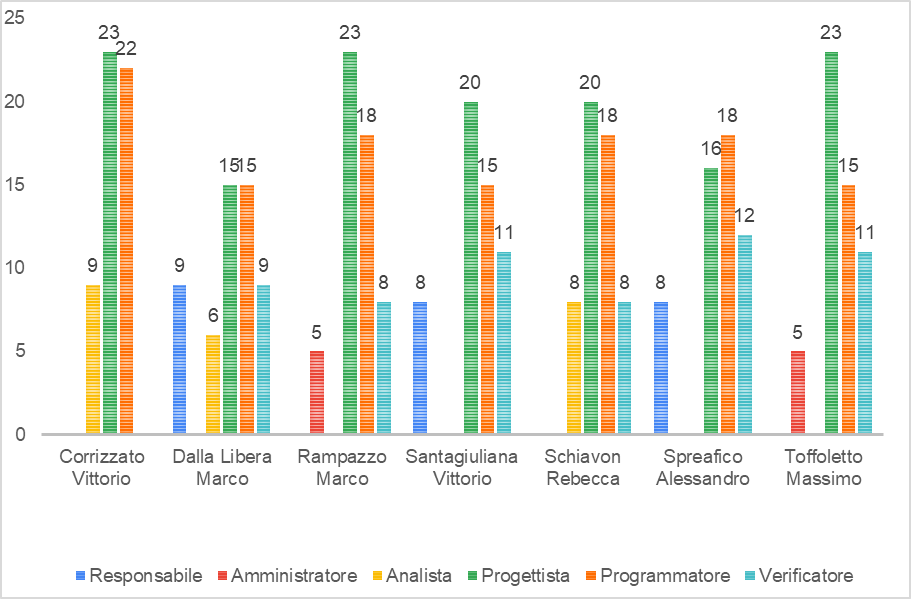
\includegraphics[width=\linewidth]{./img/Grafici/5.png}
	\caption{Grafico del prospetto orario del periodo di progettazione\glosp dettaglio e codifica}
\end{figure}
\subsubsection{Prospetto economico}
Nel periodo di progettazione\glosp dettaglio e codifica sono previsti i seguenti costi:
\begin{longtable} {
		>{}p{32mm}
		>{}p{20mm}
		>{}p{20mm}
	}
	\rowcolor{gray!50}
	
	\textbf{Ruolo} & \textbf{Ore} & \textbf{Costo} \TBstrut \\
	Responsabile & 25 & 750,00\euro{} \TBstrut \\
	Amministratore & 10 & 200,00\euro{} \TBstrut \\
	Analista & 23 & 575,00\euro{} \TBstrut \\
	Progettista & 140 & 3080,00\euro{}\TBstrut \\
	Programmatore & 121 & 1815,00\euro{} \TBstrut \\
	Verificatore & 59 & 885,00\euro{} \TBstrut \\
	\textbf{Totale} & \textbf{378}& \textbf{7305,00\euro{}} \TBstrut \\	
	\rowcolor{white}
	\caption{Prospetto economico del periodo di progettazione\glosp dettaglio e codifica}
\end{longtable} \mbox{} \\
Rappresentati nel seguente grafico: 
\begin{figure} [h!]
	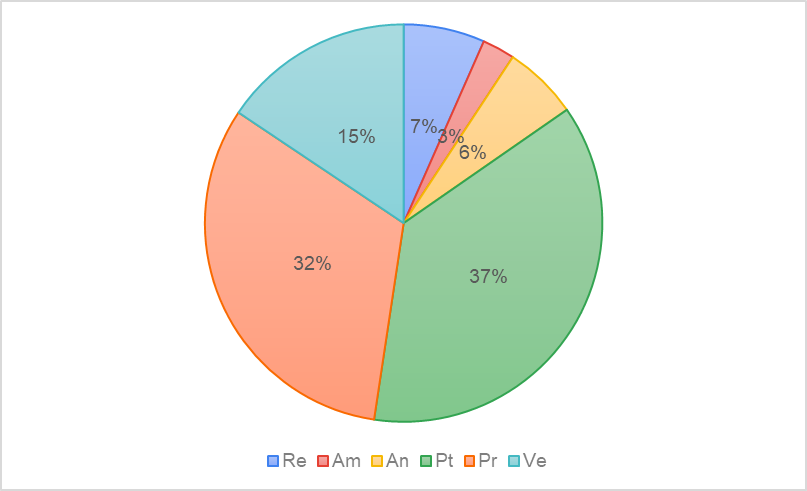
\includegraphics[width=\linewidth]{./img/Grafici/6.png}
	\caption{Grafico del prospetto economico del periodo di progettazione\glosp dettaglio e codifica}
\end{figure}

\subsection{Periodo di validazione e collaudo}
\subsubsection{Prospetto orario}
Nel periodo di validazione\glosp e collaudo è prevista la seguente divisione oraria:
\begin{longtable} {				
		>{}p{40mm}  
		>{}p{8mm}
		>{}p{8mm}
		>{}p{8mm}
		>{}p{8mm}
		>{}p{8mm}
		>{}p{8mm}
		>{}p{12mm}			
	}			
	\rowcolor{gray!50}
	\textbf{Nominativo} & \textbf{Re} & \textbf{Am} & \textbf{An} & \textbf{Pt} & \textbf{Pr} & \textbf{Ve} & \textbf{Totale}	\TBstrut \\ [2mm]
	Corrizzato Vittorio & - & - & - & - & 10 & 10 & 20 \TBstrut \\ [2mm]
	Dalla Libera Marco & 8 & 5 & - & - & 7 & - & 20 \TBstrut \\ [2mm]
	Rampazzo Marco & - & - & - & 5 & 8 & 7 & 20 \TBstrut \\ [2mm]
	Santagiuliana Vittorio & - & 5 & - & - & 6 & 9 & 20 \TBstrut \\ [2mm]
	Schiavon Rebecca & - & 8 & - & - & 7 & 5 & 20 \TBstrut \\ [2mm]
	Spreafico Alessandro & - & - & - & - & 8 & 12 & 20 \TBstrut \\ [2mm]
	Toffoletto Massimo & - & - & - & - & 9 & 11 & 20 \TBstrut \\ [2mm]
	\rowcolor{white}
	\caption{Prospetto orario del periodo di validazione\glosp e collaudo}
\end{longtable}
Rappresentata nel seguente grafico:
\begin{figure} [H]
	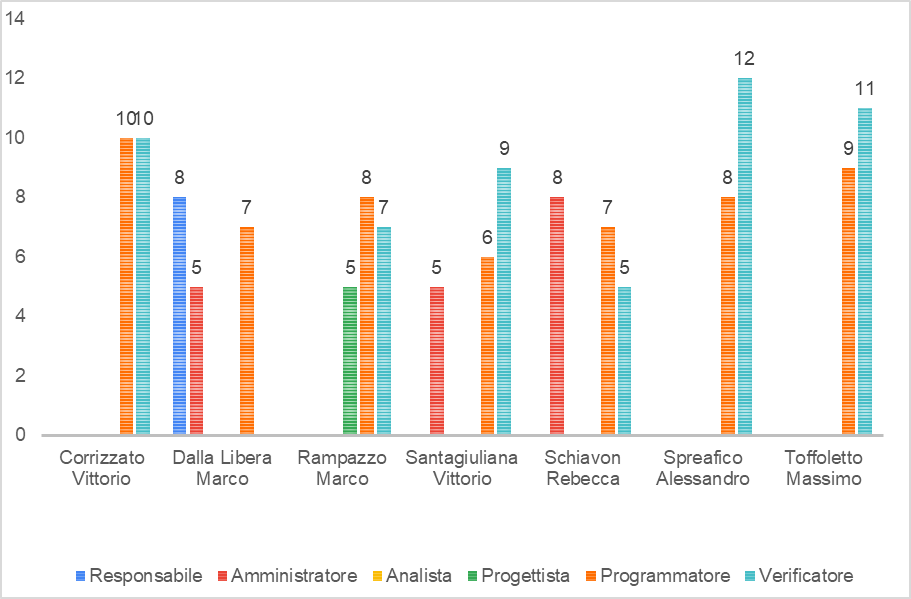
\includegraphics[width=\linewidth]{./img/Grafici/7.png}
	\caption{Grafico del prospetto orario del periodo di validazione\glosp e collaudo}
\end{figure}
\pagebreak
\subsubsection{Prospetto economico}
Nel periodo di validazione\glosp e collaudo sono previsti i seguenti costi:
\begin{longtable} {
		>{}p{32mm}
		>{}p{20mm}
		>{}p{20mm}
	}
	\rowcolor{gray!50}
	
	\textbf{Ruolo} & \textbf{Ore} & \textbf{Costo} \TBstrut \\
	Responsabile & 8 & 240,00\euro{} \TBstrut \\
	Amministratore & 18 & 360,00\euro{} \TBstrut \\
	Analista & 0 & 0,00\euro{} \TBstrut \\
	Progettista & 5 & 110,00\euro{} \TBstrut \\
	Programmatore & 55 & 825,00\euro{} \TBstrut \\
	Verificatore & 54 & 810,00\euro{} \TBstrut \\
	\textbf{Totale} & \textbf{140}& \textbf{2345,00\euro{}} \TBstrut \\	
	\rowcolor{white}
	\caption{Prospetto economico del periodo di validazione\glosp e collaudo}
\end{longtable}
Rappresentati nel seguente grafico:
\begin{figure} [H]
	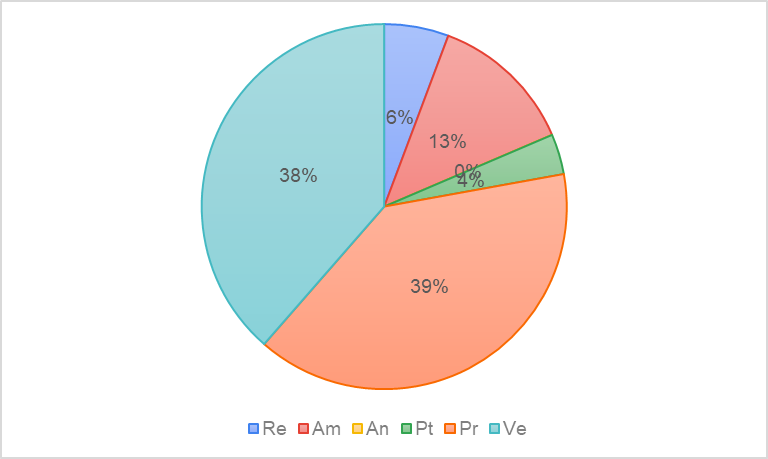
\includegraphics[width=\linewidth]{./img/Grafici/8.png}
	\caption{Grafico del prospetto economico del periodo di validazione \glosp e collaudo}
\end{figure}

\subsection{Totale ore investite}
\subsubsection{Prospetto orario}
La seguente tabella presenta la suddivisione delle ore investite per l'intero progetto\glo:
\begin{longtable} {				
		>{}p{40mm}  
		>{}p{8mm}
		>{}p{8mm}
		>{}p{8mm}
		>{}p{8mm}
		>{}p{8mm}
		>{}p{8mm}
		>{}p{12mm}			
	}			
	\rowcolor{gray!50}
	\textbf{Nominativo} & \textbf{Re} & \textbf{Am} & \textbf{An} & \textbf{Pt} & \textbf{Pr} & \textbf{Ve} & \textbf{Totale}	\TBstrut \\ [2mm]
	Corrizzato Vittorio & 6 & 6 & 23 & 33 & 37 & 22 & 127 \TBstrut \\ [2mm]
	Dalla Libera Marco & 24 & 10 & 26 & 15 & 29 & 23 & 127 \TBstrut \\ [2mm]
	Rampazzo Marco & 6 & 13 & 12 & 37 & 34 & 25 & 127 \TBstrut \\ [2mm]
	Santagiuliana Vittorio & 8 & 10 & 12 & 34 & 26 & 37 & 127 \TBstrut \\ [2mm]
	Schiavon Rebecca & 7 & 8 & 23 & 20 & 34 & 35 & 127 \TBstrut \\ [2mm]
	Spreafico Alessandro & 8 & 5 & 17 & 21 & 36 & 40 & 127 \TBstrut \\ [2mm]
	Toffoletto Massimo & 8 & 12 & 11 & 28 & 31 & 37 & 127 \TBstrut \\ [2mm]
	\rowcolor{white}
	\caption{Prospetto orario del totale di ore investite}
\end{longtable}
\pagebreak
Rappresentata anche nel seguente grafico:
\begin{figure} [H]
	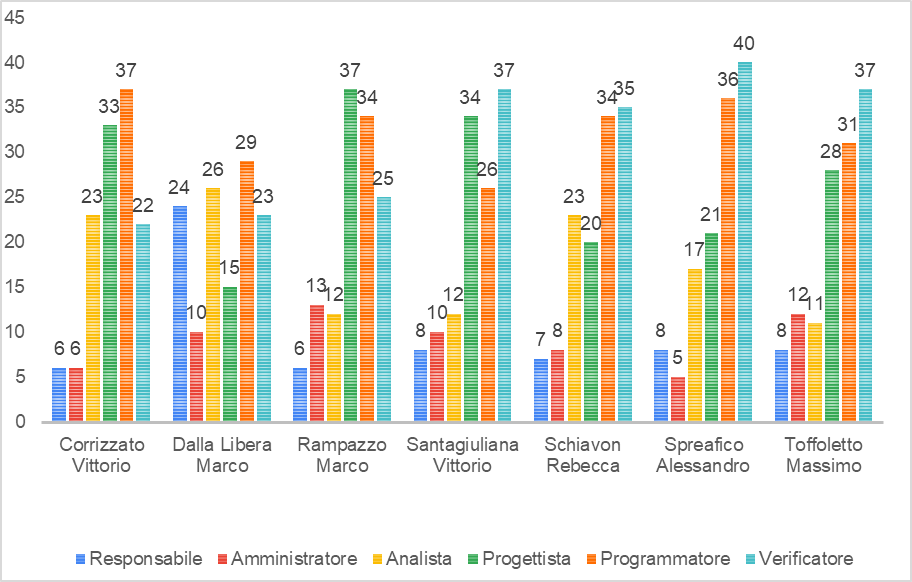
\includegraphics[width=\linewidth]{./img/Grafici/9.png}
	\caption{Grafico del prospetto orario delle ore investite per l'intero progetto\glo}
\end{figure}

\subsubsection{Prospetto economico}
La seguente tabella presenta i costi delle ore investite per l'intero progetto\glo:
\begin{longtable} {
		>{}p{32mm}
		>{}p{20mm}
		>{}p{20mm}
	}
	\rowcolor{gray!50}
	
	\textbf{Ruolo} & \textbf{Ore} & \textbf{Costo} \TBstrut \\
	Responsabile & 67 & 2010,00\euro{} \TBstrut \\
	Amministratore & 64 & 1280,00\euro{} \TBstrut \\
	Analista & 124 & 3100,00\euro{} \TBstrut \\
	Progettista & 188 & 4136,00\euro{} \TBstrut \\
	Programmatore & 227 & 3405,00\euro{} \TBstrut \\
	Verificatore & 219 & 3285,00\euro{} \TBstrut \\
	\textbf{Totale} & \textbf{749}& \textbf{17216,00\euro{}} \TBstrut \\		
	\rowcolor{white}
	\caption{Prospetto economico del totale di ore investite}
\end{longtable} \mbox{} \\ \\ \\
Rappresentati anche nel seguente grafico:
\begin{figure} [H]
	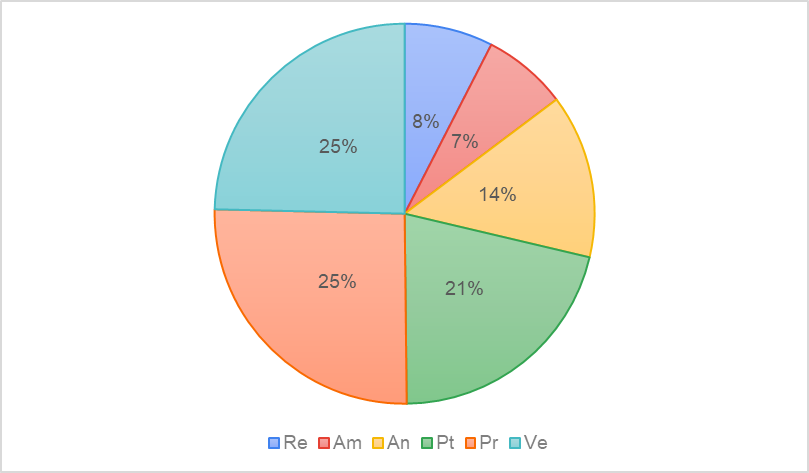
\includegraphics[width=\linewidth]{./img/Grafici/10.png}
	\caption{Grafico del prospetto economico delle ore investite per l'intero progetto\glo}
\end{figure}

\subsection{Totale ore rendicontate}
\subsubsection{Prospetto orario}
La seguente tabella presenta la suddivisione delle ore rendicontate per l'intero progetto\glo:
\begin{longtable} {				
		>{}p{40mm}  
		>{}p{8mm}
		>{}p{8mm}
		>{}p{8mm}
		>{}p{8mm}
		>{}p{8mm}
		>{}p{8mm}
		>{}p{12mm}			
	}			
	\rowcolor{gray!50}
	\textbf{Nominativo} & \textbf{Re} & \textbf{Am} & \textbf{An} & \textbf{Pt} & \textbf{Pr} & \textbf{Ve} & \textbf{Totale}	\TBstrut \\ [2mm]
	Corrizzato Vittorio & - & - & 15 & 33 & 37 & 17 & 102 \TBstrut \\ [2mm]
	Dalla Libera Marco & 17 & 10 & 13 & 15 & 29 & 18 & 102 \TBstrut \\ [2mm]
	Rampazzo Marco & 6 & 5 & - & 37 & 34 & 20 & 102 \TBstrut \\ [2mm]
	Santagiuliana Vittorio & 8 & 5 & - & 34 & 26 & 29 & 102 \TBstrut \\ [2mm]
	Schiavon Rebecca & 7 & 8 & 8 & 20 & 34 & 25 & 102 \TBstrut \\ [2mm]
	Spreafico Alessandro & 8 & 5 & 5 & 16 & 36 & 32 & 102 \TBstrut \\ [2mm]
	Toffoletto Massimo & - & 5 & 6 & 28 & 31 & 32 & 102 \TBstrut \\ [2mm]
	\rowcolor{white}
	\caption{Prospetto orario del totale di ore rendicontate}
\end{longtable}
Rappresentata anche nel seguente grafico:
\begin{figure} [H]
	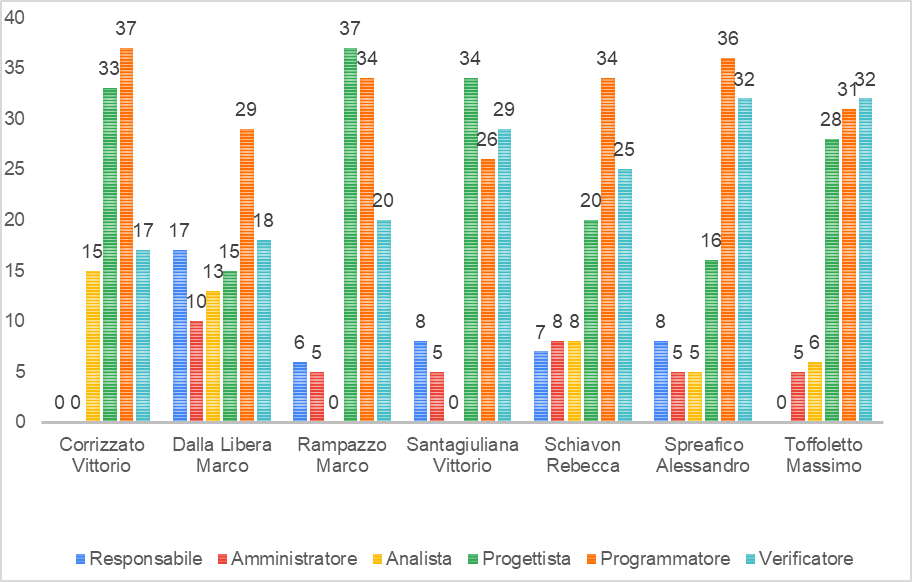
\includegraphics[width=\linewidth]{./img/Grafici/11.png}
	\caption{Grafico del prospetto orario delle ore rendicontate per l'intero progetto\glo}
\end{figure}
\pagebreak
\subsubsection{Prospetto economico}
La seguente tabella presenta i costi delle ore rendicontate per l'intero progetto\glo
\begin{longtable} {
		>{}p{32mm}
		>{}p{20mm}
		>{}p{20mm}
	}
	\rowcolor{gray!50}
	
	\textbf{Ruolo} & \textbf{Ore} & \textbf{Costo} \TBstrut \\
	Responsabile & 46 & 1380,00\euro{} \TBstrut \\
	Amministratore & 38 & 760,00\euro{} \TBstrut \\
	Analista & 47 & 1175,00\euro{} \TBstrut \\
	Progettista & 183 & 4026,00\euro{} \TBstrut \\
	Programmatore & 227 & 3405,00\euro{} \TBstrut \\
	Verificatore & 173 & 2595,00\euro{} \TBstrut \\
	\textbf{Totale} & \textbf{714}& \textbf{13341,00\euro{}} \TBstrut \\		
	\rowcolor{white}
	\caption{Prospetto economico del totale di ore rendicontate}
\end{longtable} \mbox{} \\ \\
Rappresentati anche nel seguente grafico:
\begin{figure} [H]
	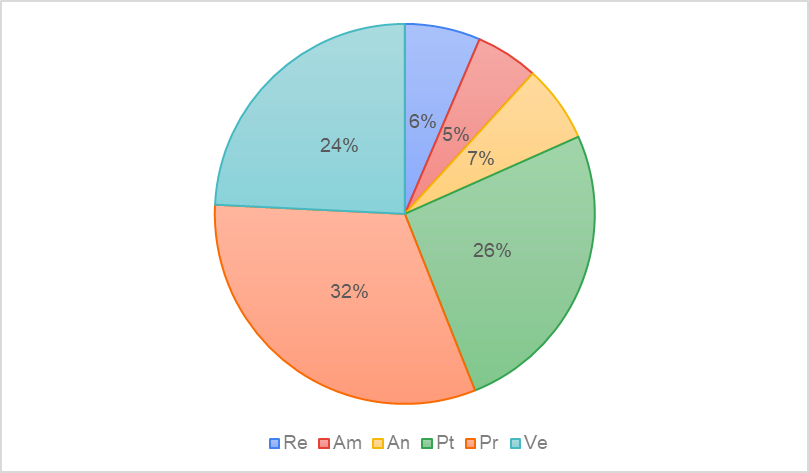
\includegraphics[width=\linewidth]{./img/Grafici/12.png}
	\caption{Grafico del prospetto economico delle ore rendicontate per l'intero progetto\glo}
\end{figure}
	
\section{Consuntivi di periodo}
Vengono riportati gli effettivi costi sostenuti per ogni periodo con le eventuali differenze rispetto a quanto preventivato. Il bilancio risulterà quindi:
\begin{itemize}
	\item \textbf{Positivo}: se i costi del consuntivo risultano minori di quelli del preventivo;
	\item \textbf{Pari}: se i costi del consuntivo risultano uguali a quelli del preventivo;
	\item \textbf{Negativo}: se i costi del consuntivo risultano superiori a quelli del preventivo.
\end{itemize}
Seguiranno quindi le conclusioni con le motivazioni delle eventuali differenze e le contromisure che il gruppo ha deciso di attuare per evitare ulteriori discrepanze con quanto dichiarato nel preventivo.
	\subsection{Periodo di Analisi}
	La tabella riporta il numero di ore effettivamente svolte dal gruppo e il rispettivo costo con le eventuali differenze rilevate rispetto al preventivo
	\begin{longtable} {							
			>{}p{40mm}  
			>{}p{20mm}	
			>{}p{28mm}			
		}			
		\rowcolor{gray!50}
		
		\textbf{Ruolo} & \textbf{Ore} & \textbf{Costo} \TBstrut \\
		Responsabile & 20(-1) & 600\euro{}(-30\euro{}) \TBstrut \\
		Amministratore & 26 & 520\euro{} \TBstrut \\
		Analista & 86(+9)& 2150\euro{}(+225\euro{}) \TBstrut \\
		Progettista & 10(+5) & 220\euro{}(+110\euro{}) \TBstrut \\
		Programmatore & 0 & 0\euro{} \TBstrut \\
		Verificatore & 46 & 690\euro{} \TBstrut \\
		\textbf{Totale Preventivo} & 175 & 3875\euro{}	\TBstrut \\	
		\textbf{Totale Consuntivo} & 188 & 4180\euro{}	\TBstrut \\	
		\textbf{Differenza Totale} & +13 & +305\euro{} \TBstrut \\
		\rowcolor{white}
		\caption{Numero di ore effettivamente svolte con rispettivo costo e differenze rispetto al preventivo}	
	\end{longtable}
	\pagebreak
	Rappresentate anche dai grafici:
	\begin{figure} [H]
		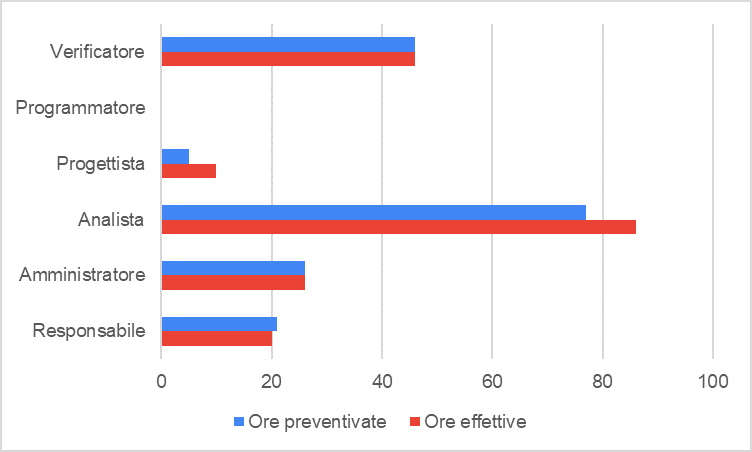
\includegraphics[width=\linewidth]{./img/Grafici/13.png}
		\caption{Grafico delle ore preventivate rispetto alle ore effettive}
	\end{figure}

	\begin{figure} [H]
		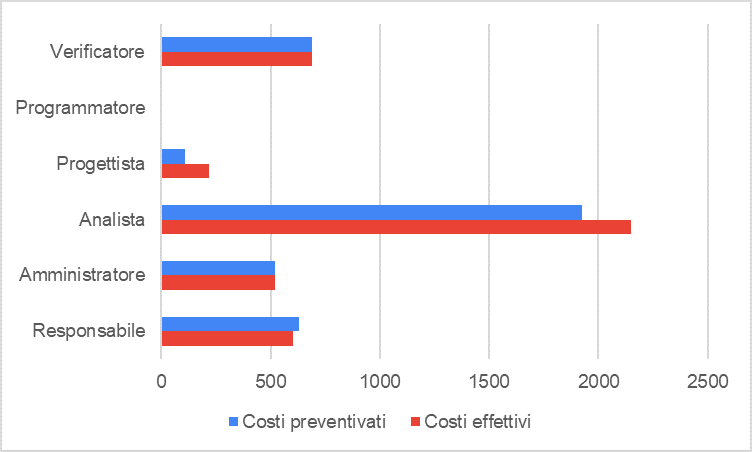
\includegraphics[width=\linewidth]{./img/Grafici/14.png}
		\caption{Grafico dei costi preventivati rispetto ai costi effettivi}
	\end{figure}

		\subsubsection{Conclusioni}
		Il bilancio risulta negativo perché le ore effettivamente svolte nei ruoli di analista, progettista e verificatore hanno superato le ore previste dal preventivo.
		Le motivazioni che hanno portato alla necessità di lavorare più del previsto sono le seguenti:
		\begin{itemize}
			\item \textbf{Analisiti}: la stesura dell'\textit{Analisi dei Requisiti} è risultata più complessa del previsto in particolare nell'individuazione dei casi d'uso\glosp e dei requisiti;
			\item \textbf{Progettisti}: sono sorte complicazioni non preventivate nella stesura del \textit{Piano di Qualifica} che hanno portato alla necessità di svolgere maggiore attività di autoapprendimento e ad un conseguente rallentamento del lavoro.
		\end{itemize}
		\subsubsection{Preventivo a finire}
		Il periodo di analisi è da intendersi come periodo di investimento per il gruppo e non viene quindi rendicontato, nel budget finale la variazione tra le ore previste e le ore effettive non provocherà alcun cambiamento. 
		È stato inoltre deciso di non modificare i successivi prospetti orari in quanto le condizioni che hanno portato alla necessità di lavorare più di quanto preventivato non dovrebbero presentarsi nuovamente. Il gruppo si ritiene ora più consapevole e meglio preparato, grazie anche alle ore di autoapprendimento già effettuate, e continua a considerare ragionevoli i prospetti orari dei prossimi periodi.
		
		\pagebreak
		\subsection{Periodo di progettazione architetturale}
		La tabella riporta il numero di ore effettivamente svolte dal gruppo e il rispettivo costo con le eventuali differenze rilevate rispetto al preventivo
		\begin{longtable} {							
				>{}p{40mm}  
				>{}p{20mm}	
				>{}p{28mm}			
			}			
			\rowcolor{gray!50}
			
			\textbf{Ruolo} & \textbf{Ore} & \textbf{Costo} \TBstrut \\
			Responsabile & 14(+1) & 420\euro (+30\euro) \TBstrut \\
			Amministratore & 13(+3) & 260\euro (+60\euro)\TBstrut \\
			Analista & 22(-2) & 550\euro (-50\euro) \TBstrut \\
			Progettista & 38 & 836\euro \TBstrut \\
			Programmatore & 58(+7) & 870\euro (+105\euro) \TBstrut \\
			Verificatore & 60 & 900\euro \TBstrut \\
			\textbf{Totale Preventivo} & 196 & 3691\euro	\TBstrut \\	
			\textbf{Totale Consuntivo} & 205 & 3836\euro	\TBstrut \\	
			\textbf{Differenza Totale} & +9 & +145\euro \TBstrut \\
			\rowcolor{white}
			\caption{Numero di ore effettivamente svolte con rispettivo costo e differenze rispetto al preventivo}	
		\end{longtable}
		Rappresentate anche dai grafici:
		\begin{figure} [H]
			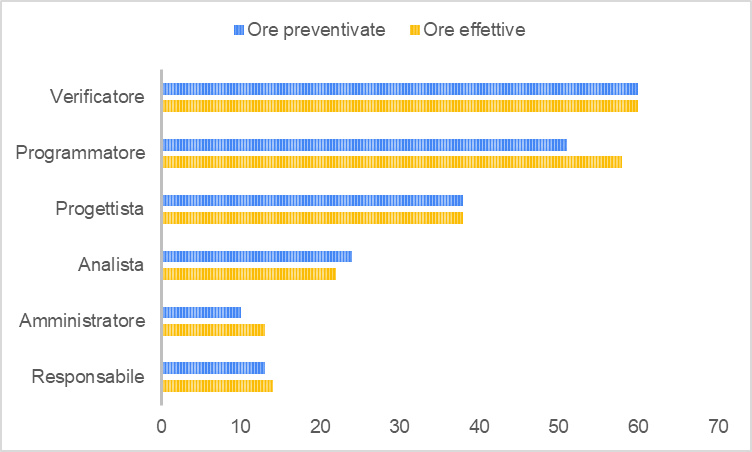
\includegraphics[width=\linewidth]{./img/Grafici/15.png}
			\caption{Grafico delle ore preventivate rispetto alle ore effettive}
		\end{figure}
		
		\begin{figure} [H]
			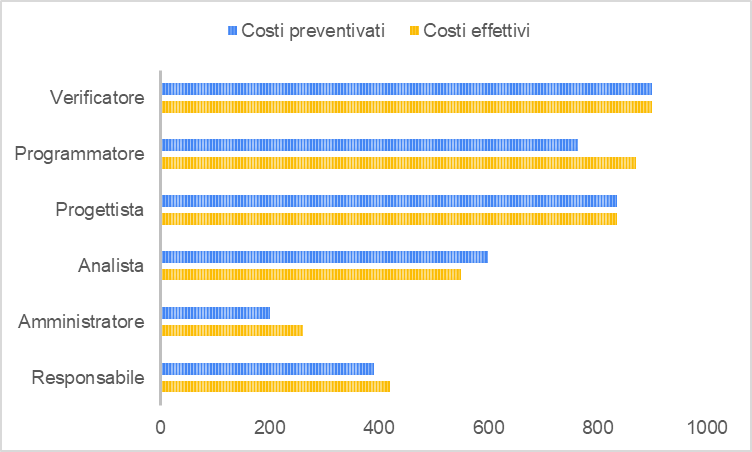
\includegraphics[width=\linewidth]{./img/Grafici/16.png}
			\caption{Grafico dei costi preventivati rispetto ai costi effettivi}
		\end{figure}
		\subsubsection{Analisi degli scostamenti}
		Al fine di garantire uno sviluppo del progetto\glosp congruo con quanto preventivato nei tempi e nei costi, al termine di ogni periodo individuato nella pianificazione si rilevano eventuali problemi riscontrati ed eventualmente si modifica e si dettaglia ulteriormente la pianificazione futura in modo da mitigare gli effetti di questi imprevisti.
		\paragraph*{I periodo} \mbox{} \\
		Il tempo dedicato alla revisione e all'aggiornamento delle \textit{Norme di Progetto} è risultato insufficiente, è stato quindi necessario prolungare quest'attività anche per il secondo periodo.
		Ciò ha causato un aumento delle ore del ruolo dell'amministratore.
		\paragraph*{II periodo} \mbox{} \\
		Al termine del secondo periodo non è stata individuata nessuna complicazione. Nonostante si sia dovuta rivedere la pianificazione vista la necessità di inserire anche in questo periodo l'attività di revisione e aggiornamento delle \textit{Norme di Progetto}, non sono stati rilevati ritardi o imprevisti oltre all'aumento delle ore per il ruolo dell'amministratore come già indicato. È stata quindi mantenuta la pianificazione prevista per il III periodo.
		\paragraph*{III periodo} \mbox{} \\
		È stato rilevato che l'attività di ricerca di strumenti e tecnologie svolta nel I periodo non è stata affiancata da un sufficiente studio degli strumenti e delle tecnologie individuate. Questo ha portato alla necessità di svolgere dell'autoapprendimento da parte di due componenti del gruppo che hanno poi illustrato quanto appreso agli altri membri. Di conseguenza si è verificato un ritardo nel ruolo dei programmatori. Questo ritardo, tuttavia, non è stato così rilevante da non permettere la codifica del proof of concept\glosp come da pianificazione, non è stato quindi necessario nessun cambiamento sulla pianificazione futura. 
		\paragraph*{IV periodo} \mbox{} \\
		Grazie all'attività di autoapprendimento svolta nel III periodo non ci sono stati problemi o ritardi nel IV periodo.
		\paragraph*{V periodo} \mbox{} \\
		Non sono stati rilevati scostamenti dalla pianificazione del V periodo.
		\subsubsection{Conclusioni}
		Il bilancio risulta negativo perché le ore effettivamente svolte nei ruoli di responsabile, amministratore e programmatore hanno superato le ore previste dal preventivo.
		Le motivazioni che hanno portato alla necessità di lavorare più del previsto sono le seguenti:
		\begin{itemize}
			\item \textbf{Responsabile}: per cause esterne all'ambito universitario è stato impossibile svolgere alcuni incontri previsti ed è stata necessaria una conseguente riorganizzazione delle modalità di incontro, ciò ha portato ad un inatteso aumento del lavoro per il responsabile;
			\item \textbf{Amministratore}: è sorta la necessità di utilizzare strumenti e tecnologie inizialmente non previsti, la necessità di normare l'utilizzo di quest'ultimi ha rallentato la revisione e l'aggiornamento delle \textit{Norme di Progetto} richiedendo un aumento delle ore lavorative per l'amministratore;
			\item \textbf{Programmatore}: è stato necessario uno studio più approfondito delle tecnologie rispetto a quanto non era già stato preventivato, ciò ha causato la necessità di un numero maggiore di ore anche per i programmatori.
		\end{itemize}
		Le contromisure attuate per mitigare i problemi riscontrati sono indicate nell'analisi degli scostamenti e nelle tabelle di attuazione dei rischi.
		\subsubsection{Preventivo a finire}
		Il bilancio risulta negativo in quanto i costi effettivi superano quelli preventivati. Per fronteggiare questo problema verrà modificata la pianificazione futura in modo da presentarci ai proponenti con un preventivo finale il più aderente possibile a quello iniziale. 
